\documentclass[12pt, a4paper]{article}
\usepackage[ebgaramond]{fontsetup}
    % \usepackage[lining,semibold,scaled=1.05]{ebgaramond} % font
    \usepackage[T1]{fontenc}
    \usepackage{fullpage}
    \usepackage{amsmath}
    \usepackage{amssymb}
    \usepackage{textcomp}
    \usepackage[utf8]{inputenc}
    \usepackage[margin=1in]{geometry}
    \usepackage{fontawesome}
    \usepackage{etoolbox}
    \usepackage{booktabs}
    \usepackage{array}


    \usepackage{latexsym}
    \usepackage{titlesec}
    \usepackage{marvosym}
    \usepackage[usenames,dvipsnames]{color}
    % sepackage{verbatim}
    \usepackage{enumitem}
    \usepackage{amssymb}
    \usepackage[hidelinks]{hyperref}
    \usepackage{fancyhdr}
    \usepackage[english]{babel}
% image
    \usepackage[all]{background}

    \input{glyphtounicode}
    \textheight=11in
    \pagestyle{empty}
    \raggedright


% page format commands %

\pagestyle{fancy}
\fancyhf{} % clear all header and footer fields
\fancyfoot{}
\renewcommand{\headrulewidth}{0pt}
\renewcommand{\footrulewidth}{0pt}

% column space
\setlength{\tabcolsep}{52pt}

% Adjust margins
\addtolength{\oddsidemargin}{-0.5in}
\addtolength{\evensidemargin}{-0.5in}
\addtolength{\textwidth}{1in}
\addtolength{\topmargin}{-.5in}
\addtolength{\textheight}{1.0in}

\urlstyle{same}

\raggedbottom
\raggedright
\setlength{\tabcolsep}{0in}

\newcolumntype{R}[1]{>{\raggedleft\arraybackslash}p{#1}} % Define a new right-aligned column type
\newcolumntype{L}[1]{>{\raggedright\arraybackslash}p{#1}} % Define a new left-aligned (no justification) column type
\newcolumntype{C}[1]{>{\centering\arraybackslash}p{#1}} % Define a new centred column type

% Sections formatting
\titleformat{\section}{
  \vspace{-4pt}\scshape\raggedright\large
}{}{0em}{}[\color{black}\titlerule \vspace{-5pt}]

% Ensure that generate pdf is machine readable/ATS parsable
\pdfgentounicode=1

\def\bull{\vrule height 0.8ex width .7ex depth -.1ex }

%-------------------------
% Custom commands
\newcommand{\resumeItem}[1]{
  \item\small{
    {#1 \vspace{-2pt}}
  }
}

\newcommand{\resumeSubheading}[4]{
  \vspace{-2pt}\item
    \begin{tabular*}{0.97\textwidth}[t]{l@{\extracolsep{\fill}}r}
      \textbf{#1} & #2 \\
      \textit{\small#3} & \textit{\small #4} \\
    \end{tabular*}\vspace{-7pt}
}

\newcommand{\resumeSubSubheading}[2]{
    \item
    \begin{tabular*}{0.97\textwidth}{l@{\extracolsep{\fill}}r}
      \textit{\small#1} & \textit{\small #2} \\
    \end{tabular*}\vspace{-7pt}
}

\newcommand{\resumeProjectHeading}[2]{
    \item
    \begin{tabular*}{0.97\textwidth}{l@{\extracolsep{\fill}}r}
      \small#1 & #2 \\
    \end{tabular*}\vspace{-7pt}
}

\newcommand{\resumeSubItem}[1]{\resumeItem{#1}\vspace{-4pt}}

\renewcommand\labelitemii{$\vcenter{\hbox{\tiny$\blacksquare$}}$}

\newcommand{\resumeSubHeadingListStart}{\begin{itemize}[leftmargin=0.15in, label={}]}
\newcommand{\resumeSubHeadingListEnd}{\end{itemize}}
\newcommand{\resumeItemListStart}{\begin{itemize}} %[topsep=0pt,itemsep=0pt,parsep=0pt,before=\vspace{0cm},after=\vspace{1mm}] % added option to save space
\newcommand{\resumeItemListEnd}{\end{itemize}\vspace{-16pt}}

%-------------------------------------------

% DEFINITIONS FOR RESUME %%%%%%%%%%%%%%%%%%%%%%%

\newcommand{\area} [2] {
    \vspace*{-9pt}
    \begin{verse}
        \textbf{#1}   #2
    \end{verse}
}

\newcommand{\lineunder} {
    \vspace*{-8pt} \\
    \hspace*{-18pt} \hrulefill \\
}

\newcommand{\header} [1] {
    {\hspace*{-18pt}\vspace*{6pt} \textsc{#1}}
    \vspace*{-6pt} \lineunder
}

\newcommand{\employer} [3] {
    { \textbf{#1} (#2)\\ \underline{\textbf{\emph{#3}}}\\  }
}

\newcommand{\contact} [3] {
    \vspace*{-10pt}
    \begin{center}
        {\Huge \scshape {#1}}\\
        #2 \\ #3
    \end{center}
    \vspace*{-8pt}
}

\newenvironment{achievements}{
    \begin{list}
        {$\bullet$}{\topsep 0pt \itemsep -2pt}}{\vspace*{4pt}
    \end{list}
}

\newcommand{\schoolwithcourses} [4] {
    \textbf{#1} #2 $\bullet$ #3\\
    #4 \\
    \vspace*{5pt}
}

\newcommand{\school} [4] {
    \textbf{#1} #2 $\bullet$ #3\\
    #4 \\
}
% END RESUME DEFINITIONS %%%%%%%%%%%%%%%%%%%%%%%

\usepackage{garamondlibre}

% ====PIC====
\newcommand{\MyGraphicLogo}{% For imported graphic logo
\begin{tikzpicture}[remember picture,overlay,yshift=-2cm, xshift=-2cm]
  \node at (0,0) {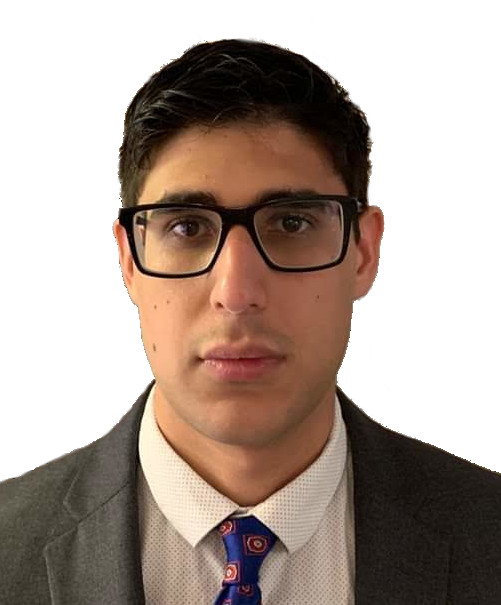
\includegraphics[width=3cm]{suitpic.jpg}};
 \end{tikzpicture}
}
\SetBgContents{\MyGraphicLogo}% Select tikz picture

\SetBgPosition{current page.north east}% Select location
\SetBgOpacity{1.0}% Select opacity
\SetBgAngle{0.0}% Select roation of logo
\SetBgScale{1.0}% Select scale factor of logo

\begin{document}

%==== HEADER ====%
\vspace*{-12pt}
\begin{center}
	{\Huge \scshape {Alex Diaz}}\\
	\vspace{1mm}
	\faMapMarker \hspace{.5mm} Tokyo, Japan $\cdot$ 
	\faEnvelope \hspace{.5mm} \href{mailto:alejandrojsdiaz@outlook.com}{alejandrojsdiaz@outlook.com} $\cdot$ \faMobile \hspace{.5mm} +81 080-7266-8529
		
	\faGithub \hspace{.5mm} \href{https://github.com/calmcoconut}{GitHub} $\cdot$
	\faLinkedin \hspace{.5mm} \href{https://www.linkedin.com/in/diazjalejandro/}{LinkedIn} $\cdot$
	\faTwitter \hspace{.5mm} \href{https://twitter.com/greetingsfriend}{Twitter} $\cdot$
    \faBriefcase \hspace{.5mm} \href{https://calmcoconut.github.io/diasDiaz/}{My website}
    \\
\end{center}


%==== Education ====%
\section{Education}
  \resumeSubHeadingListStart
    \resumeSubheading
      {Georgia Institute of Technology}{Atlanta, GA}
      {Master of Science in Computer Science}{Jan. 2021 -- May 2024}
    \resumeSubheading
      {The University of Georgia}{Athens, GA}
      {Bachelor of Arts in Economics, Minor in History}{Aug. 2013 -- May 2017}
 \resumeSubHeadingListEnd

 %-----------EXPERIENCE-----------
\section{Experience}

\resumeSubHeadingListStart
  \resumeSubheading
    {Software Engineering Tutor}{Feb 2020 -- Present}
    {FDS Services}{Tokyo, Japan}
    \resumeItemListStart
      \resumeItem{Teaching students engineering practices and fundamentals of \textbf{Java}, \textbf{Python}, MIT Scratch, and \textbf{OO} design}
    \resumeItemListEnd
    \resumeSubHeadingListEnd

\resumeSubHeadingListStart
  \resumeSubheading
    {Data Analyst Manager}{Nov 2018 -- Nov 2019}
    {United Parcel Service (UPS)}{Sandy Springs, GA}
    \resumeItemListStart
      \resumeItem{Assembled and developed automated data reporting for executive leadership in US sales Vice President and President with \textbf{SQL}, \textbf{Python's Pandas}, and \textbf{Power BI}}
      \resumeItem{Oversaw inter-team coordination to automate reporting practices. Reduced daily reporting workloads from 3 hours to 3 minutes by automating reports using Python and Microsoft \textbf{VBA} with \textbf{SQL} database}
      \resumeItem{Implemented SQL server database jobs to minimizing manual maintenance and reporting requirements}
      \resumeItem{Addressed production bugs and made improvements in existing inter-team reporting in \textbf{Python}, \textbf{VBA}, and \textbf{SQL}}
    \resumeItemListEnd
    \resumeSubHeadingListEnd

\resumeSubHeadingListStart
  \resumeSubheading
    {Data Analyst Volunteer}{July 2018 -- Sept 2018}
    {Bredesen for Tennessee Senate}{Nashville, TN remote}
    \resumeItemListStart
      \resumeItem{Created data visualizations to impact voter turnout with \textbf{Tableau}}
      \resumeItem{Generated weekly reports using \textbf{SQL, Excel pivot tables,} and \textbf{VBA macros}; provided \textbf{metric reporting}}
      \resumeItem{Presented analytical data to multiple teams, demonstrating analytical data to add value to on-the-ground efforts}
    \resumeItemListEnd
\resumeSubHeadingListEnd

%adding some space%
\vspace{2pt}


% -----------Multiple Positions Heading-----------
%    \resumeSubSubheading
%     {Software Engineer I}{Oct 2014 - Sep 2016}
%     \resumeItemListStart
%        \resumeItem{Apache Beam}
%          {Apache Beam is a unified model for defining both batch and streaming data-parallel processing pipelines}
%     \resumeItemListEnd
%    \resumeSubHeadingListEnd
%-------------------------------------------

%==== Independent projects ====%
\section{Projects}
\textbf{IQ AI agent} | \small\textit{Python, NumPy, PIL, Docker, OpenCV}
\begin{itemize}[noitemsep,topsep=0pt]
  \item Undertook implementing an AI that solves the Raven's Progressive Matrix IQ
  \item Demonstrated performance and problem-solving creativity comparable to a human test taker
  \item Used \textbf{Computer Vision} algorithms via \textbf{OpenCV} and \textbf{NumPy}
\end{itemize}

\textbf{TimeTime} Android Application | \small\textit{Java, Kotlin, Android Jetpack, Android Material, Room DB, Java Thread}
\begin{itemize}[noitemsep,topsep=0pt]
  \item Created a time logging Android Application following a MVC design pattern supported by Android's Room persistent database design
\end{itemize}

\textbf{Spotify Music Advisor} | \small\textit{Java, Spring, HTTP, OAuth2, JSON}
\begin{itemize}[noitemsep,topsep=0pt]
  \item Implemented a RESTful server capable of OAuth handshake and authentication with Spotify
\end{itemize}

\section{Technical Skills}
\textbf{Languages:} Java, Kotlin, Python, C/C++, Golang, SQL, HTML/CSS, Bash \\
\textbf{Frameworks} \& \textbf{Libraries:} Spring, JUnit, Guava, Flask, Android, NumPy, Pandas, OpenCV \\
\textbf{Dev Tools:} Git, Agile, Google Cloud, AWS, VIM, Docker, Linux \\
\textbf{Misc:} Test-driven development, PASSED---CFA LV 1, Human-Computer Design

\end{document}
